\section{Baseline Calibration {\color{blue} Laurence} }
%\label{se:baseline_calibration}

\subsection{Methodology}
Calibration factors are estimated from a series of OTF scans towards Uranus

\subsection{Data sets}

\addparag{ selected scan numbers}

Uranus measured-to-predicted flux density ratios are shown in Fig.~\ref{fig:uranus_flux_fwhm} as a fonction of the 2D Gaussian FWHM estimates and color-coded from the observation dates given in UT hours. As discussed in Sect.~\ref{se:obsdate_variations}, a correlation between the flux densities and the FWHM estimates is observed, broaden beams are associated with lower fluxes. However, the baseline scan selection, discussed in Sect.~\ref{se:data_selection}, which relies on the observation date among other criteria, is efficient to discard the larger beam scans, and thus mitigates the flux dispersion.          


\begin{figure}[ht!]
\begin{center}
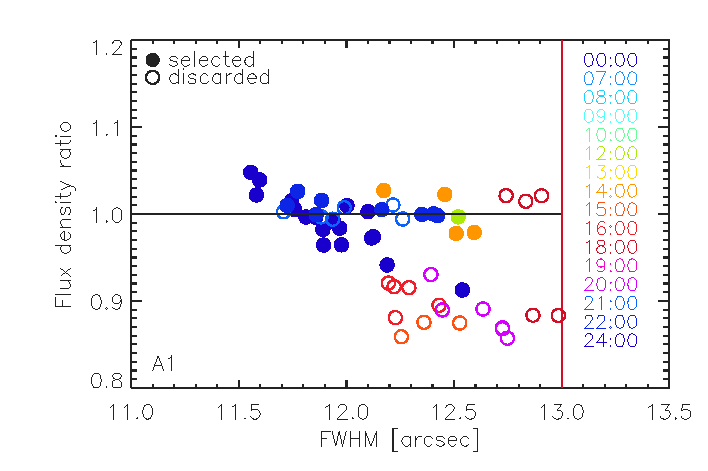
\includegraphics[clip=true,width=0.47\textwidth]{Figures/Calibration/plot_flux_density_ratio_primary_a1.pdf}
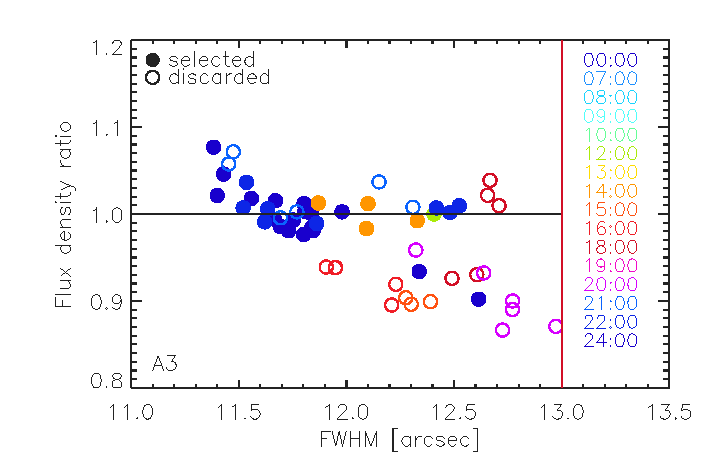
\includegraphics[clip=true,width=0.47\textwidth]{Figures/Calibration/plot_flux_density_ratio_primary_a3.pdf}
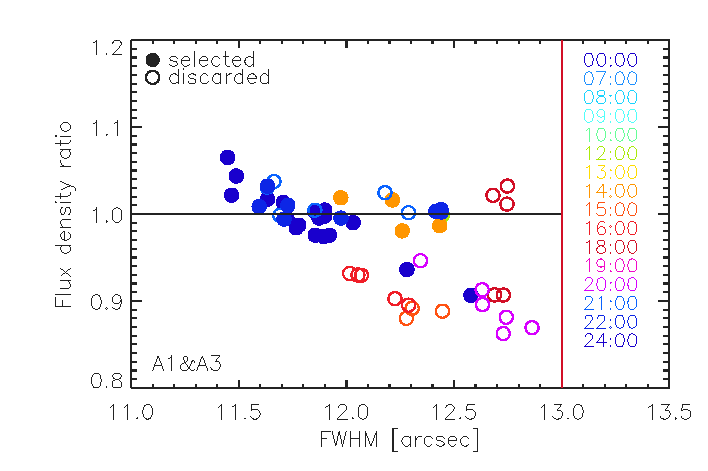
\includegraphics[clip=true,width=0.47\textwidth]{Figures/Calibration/plot_flux_density_ratio_primary_1mm.pdf}
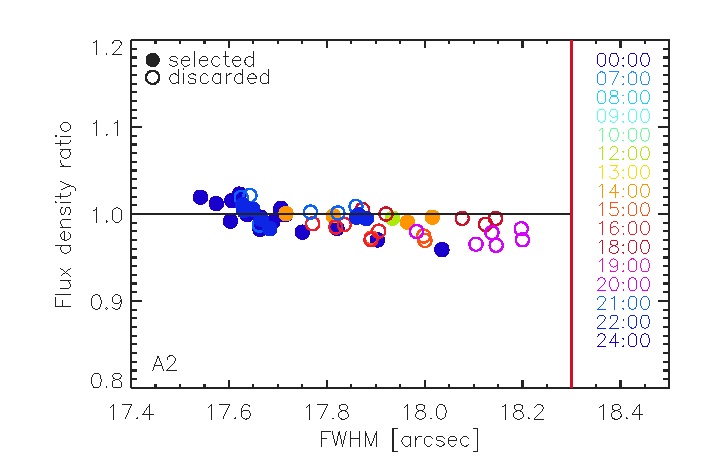
\includegraphics[clip=true,width=0.47\textwidth]{Figures/Calibration/plot_flux_density_ratio_primary_a2.pdf}
\caption[Uranus flux density stability against FWHM]{Ratio of the
  Uranus measured flux densities to expectations in fonction of the
  measured 2D
  Gaussian beam FWHM for array 1 (upper left), array 3 (upper right),
  1mm array combination (lower left) and array 2 (lower right),
  including scans acquired during N2R9, N2R12 and N2R14 campaigns. The
  color code indicates the range of observing time in UT hours, shades
  of blue corresponds to night time observations while shades of red
  to day time. A primary scan selection is performed from measured
  opacity criteria, as defined in Sect.~\ref{se:data_selection}, and
  from FWHM estimates, where the FWHM thresholds are showed as red vertical
  lines. The scans that met the baseline selection criteria (see
  Sect.~\ref{se:data_selection})
  are shown as filled circled, whereas the discarded scans are open circles.}
\label{fig:uranus_flux_fwhm}
\end{center}
\end{figure}


\subsection{Stability against the observed opacity}

\addparag{ stability against opacity}

\begin{figure}[ht!]
\begin{center}
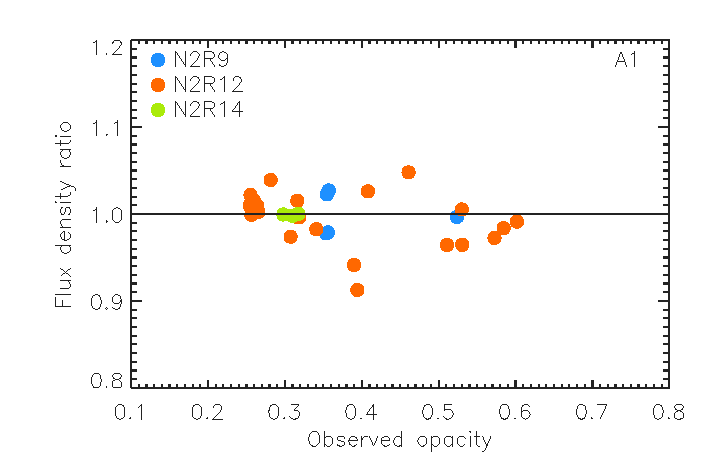
\includegraphics[clip=true,width=0.47\textwidth]{Figures/Calibration/plot_flux_density_ratio_obstau_primary_a1.pdf}
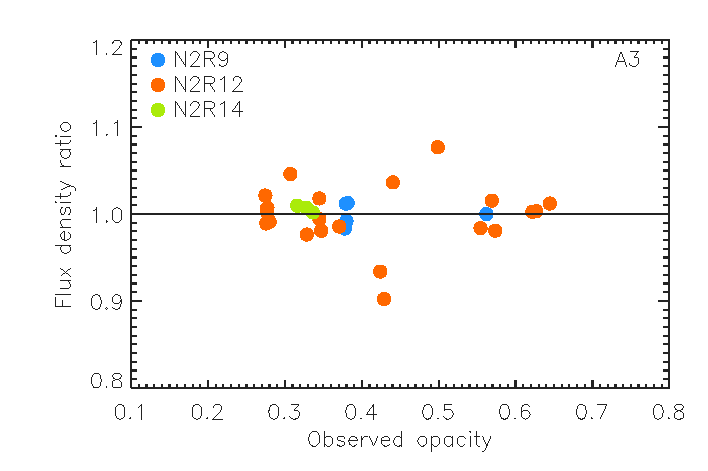
\includegraphics[clip=true,width=0.47\textwidth]{Figures/Calibration/plot_flux_density_ratio_obstau_primary_a3.pdf}
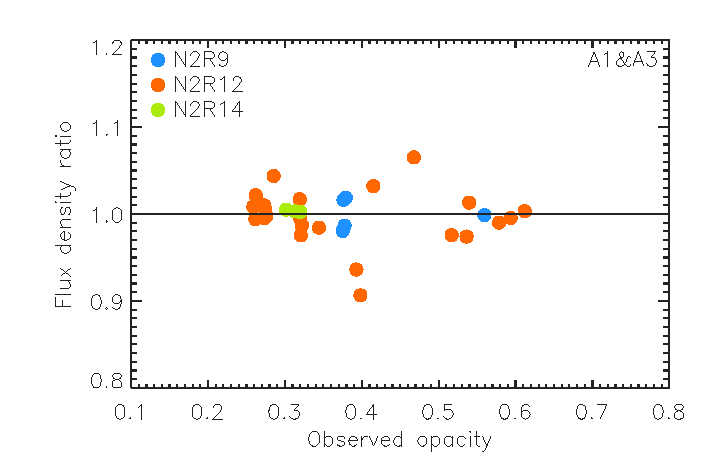
\includegraphics[clip=true,width=0.47\textwidth]{Figures/Calibration/plot_flux_density_ratio_obstau_primary_1mm.pdf}
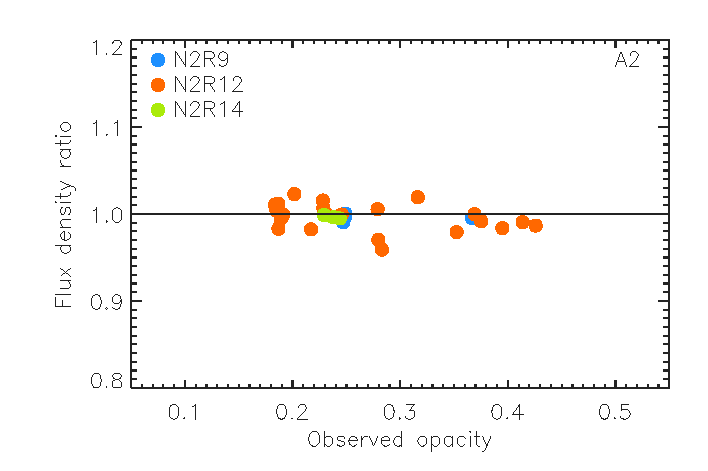
\includegraphics[clip=true,width=0.47\textwidth]{Figures/Calibration/plot_flux_density_ratio_obstau_primary_a2.pdf}
\caption[Uranus flux density stability against observed
  opacity]{Uranus measured-to-modeled flux density ratio as a fonction
  of the measured observed opacity for array 1 (upper left), array 3
  (upper right), 1mm array combination (lower left) and array 2 (lower
  right). The datapoints denote the flux ratio of the scans retained after the
  baseline section is performed, for the three campaigns, N2R9
  in blue, N2R12 in orange and N2R14 in chartreuse (yellow green). For
  each campaign, flux ratios are equal to unity in average by
  construction and are stable againts the observed opacity, modelled as
  the zenith opacity times the air mass at the telescope elevation.}
\label{fig:uranus_flux_obstau}
\end{center}
\end{figure}
